\subsection{Q10.14 data 10312021 grouped by scenario}

\begin{comment}
            EFPR        EO      EFNR     n    pvalue
frauth  0.380952  0.619048  0.380952  21.0  0.169213
icu     0.500000  0.500000  0.500000  19.0  0.868534
rent    0.357143  0.642857  0.357143  21.0  0.143411
\end{comment}

\begin{table}[h]
    \centering
    \begin{tabular}{|c|c|c|c|c|c|}
        \hline
        scenario & EFPR & EO & EFNR & n & p-value\\
        \hline
        frauth & 0.381 & \textbf{0.619} & 0.381 & 21.0 & 0.169\\
		icu & 0.500 & 0.500 & 0.500 & 19.0 & 0.869\\
		rent & 0.357 & \textbf{0.643} & 0.357 & 21.0 & 0.143\\
		
        \hline
    \end{tabular}
    \caption{Grouped by scenario}
    \label{tab:my_label}
\end{table}
\begin{figure}[h]
    \centering
    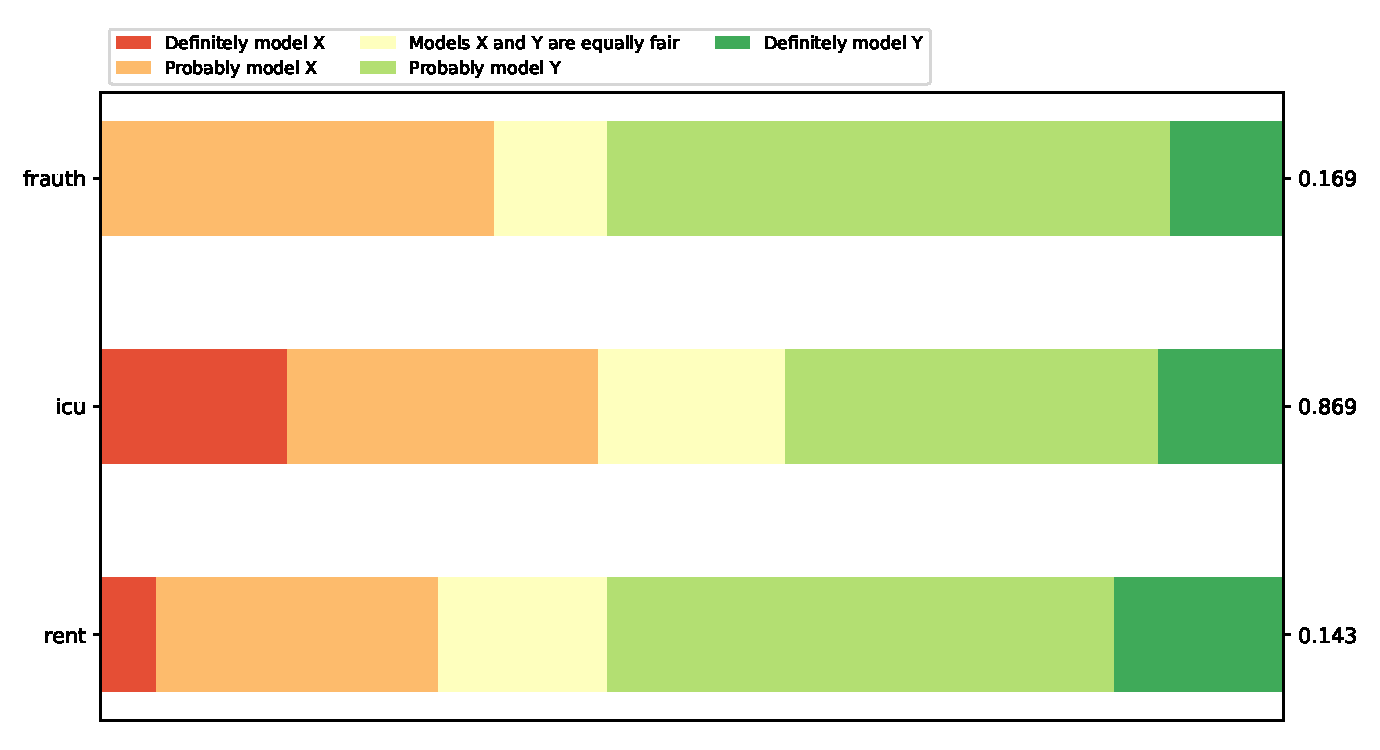
\includegraphics[width=0.8\textwidth]{figures/Q10.14/10312021/Q10.14_scenario.pdf}
    \caption{Grouped by scenario}
    \label{fig:my_label}
\end{figure}
